\chapter{Methodology}
\label{chap:methodology}

In order to address the research questions, we need to develop a proof of concept system that is able to investigate and utilize the concepts in question. It was decided that a to-do list application would be a good candidate for investigating these concepts. A to-do list application is a task management system in a simple form. The simplest version of it could be just a list of strings representing the user's tasks, or to-do items, that needs to be done. Another form of a task management system is a calendar. A calendar would also be a suitable candidate for looking into the use of contexts in task management. However, a calendar is more complex than a to-do list, even in its simplest form, and would require more design decisions than a to-do list if building a system from scratch. Considering this, a to-do list application was chosen.

When building context-aware systems, the most natural choice of platform is mobile devices. Contextual information is readily available on such devices because of their cheap and integrated sensors, which now exists on nearly all modern handheld devices. It is easy to access information such as user activity, time and location. The two most popular operating systems for such devices are Android and iOS. The development frameworks for both of these have functionality that allows for easy acquirement of context data. Even context abstraction and representation are handled by the frameworks, so that the developer no longer has to deal with the raw sensory data coming from the hardware. For this particular thesis, the Android Operating System was chosen for development. This is mostly because it holds the biggest market share by far, but also because an Android device was easily available for development.




\section{User group}
For the recommender to be able to differ between user tasks, these tasks needs to be assigned different types and be categorized. However, categorizing typical and everyday tasks will require a lot of effort. It is known that modeling an individual's tasks and activities can be challenging \cite{refanidis2010constraint}. Consider trying to generalize the tasks of an office worker and a carpenter. The tasks that these two typically do during a day, will vary greatly. Finding similarities among these tasks so that they could be generalized to fit a general population would be difficult. Therefore, in order to reduce complexity and the amount of work needed, it was decided that the scope should be narrowed down by selecting a specific user group. This will also allow for narrowing down the application itself, both in terms of general application design as well as the complexity of context collection and representation.

The user group that was selected was students, and more specifically students in an educational environment. There were two main reasons for this. One being that the tasks of such a narrowed down and specific user group can be much easier divided into separate types and categorized. We will then be able to predefine a set of tasks that should cover most of the different types of tasks that a student will be doing in an educational environment. The second reason for choosing students was that this user group was easily accessible for questioning or experimenting.

Although students were selected as the target user group, typical educational tasks can still vary to a large degree between undergraduate and postgraduate students. This can also be highly dependent on what semester the student in question is currently in. A bachelor student might have very different tasks than a master student doing his/hers master thesis. To determine these differences, and to find out whether or not eventual differences needed to be accounted for in the application design, a short questionnaire was made. Detailed results of the questionnaire can be found in Section~\ref{subsec:studenttasks}. Through the questionnaire, we found that there were only minor differences between the tasks of the different types of students. It was therefore decided that the tasks should be categorized equally for all students.

The actual task categories used for the tasks in the application were:
\begin{itemize}
	\item Attend lecture
	\item Read
	\item Write report
	\item Do course exercises
	\item Meeting
	\item Group work
	\item Practical work
	\item Other
\end{itemize}
These categories are based on the results of the short student task questionnaire we made. We provided a set of predefined tasks where the student had to answer how often they typically performed each task, both in terms of regularity (once a day, once a week etc.) and frequency (1-3 times a week, 4-6 times a week etc.). They students were also able to fill in additional tasks, if the predefined tasks were not enough to cover all the tasks that they typically do.



\section{Application}

\subsection{General application design}
By choosing to create a todo-list application the user should be able to perform actions that are normal for such applications. These actions include creating and storing tasks, as well editing and deleting them. The tasks should also be possible to arrange into lists. The application in this study is developed in a way that supports all these aspects. When a todo-item or task is created, a date will be attached to that particular task, thereby organizing the tasks with similar dates into lists.

We would also need a schema for storing context information, as well as a recommender that will process the stored contexts and provide recomendations. A conceptual model of the application is shown in Figure~\ref{fig:conceptualmodel}.
\begin{figure}[tbp]
  \centering
  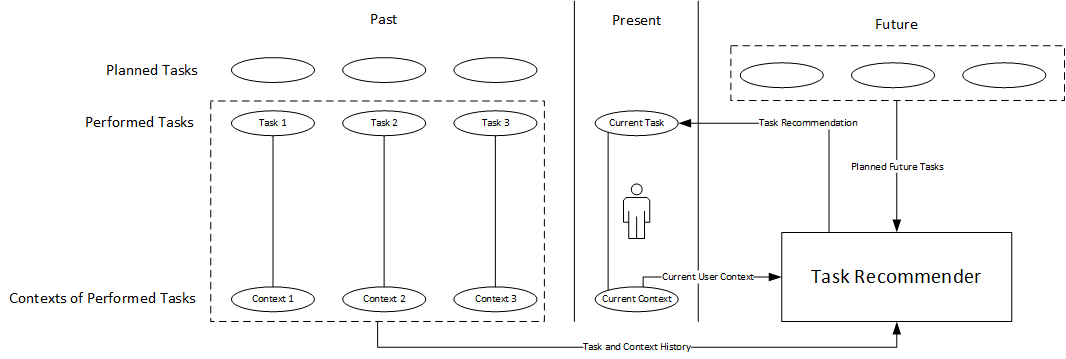
\includegraphics[width=\textwidth]{figures/ConceptualDiagram.png}
  \caption[Conceptual model]{Conceptual model of the application.}
  \label{fig:conceptualmodel}
\end{figure}
The lines pointing towards the recommender represents its input, whereas the line pointing outward is the actual recommendation. The input for the recommender consists of three parts:
\begin{itemize}
	\item The tasks that the user needs to do (planned tasks).
	\item The tasks that the user has previously done (task history).
	\item The contexts of related to the previously done tasks (context history).
	\item The users current context.
\end{itemize}
By taking all these components into account, the recommender will be able process the information and suggest a task for the user. The recommender is discussed more thoroughly in Section~\ref{sec:recommender}.

The design of the main application screen is shown in Figure~\ref{fig:designmainscreen}.
\begin{figure}[tbp]
  \centering
  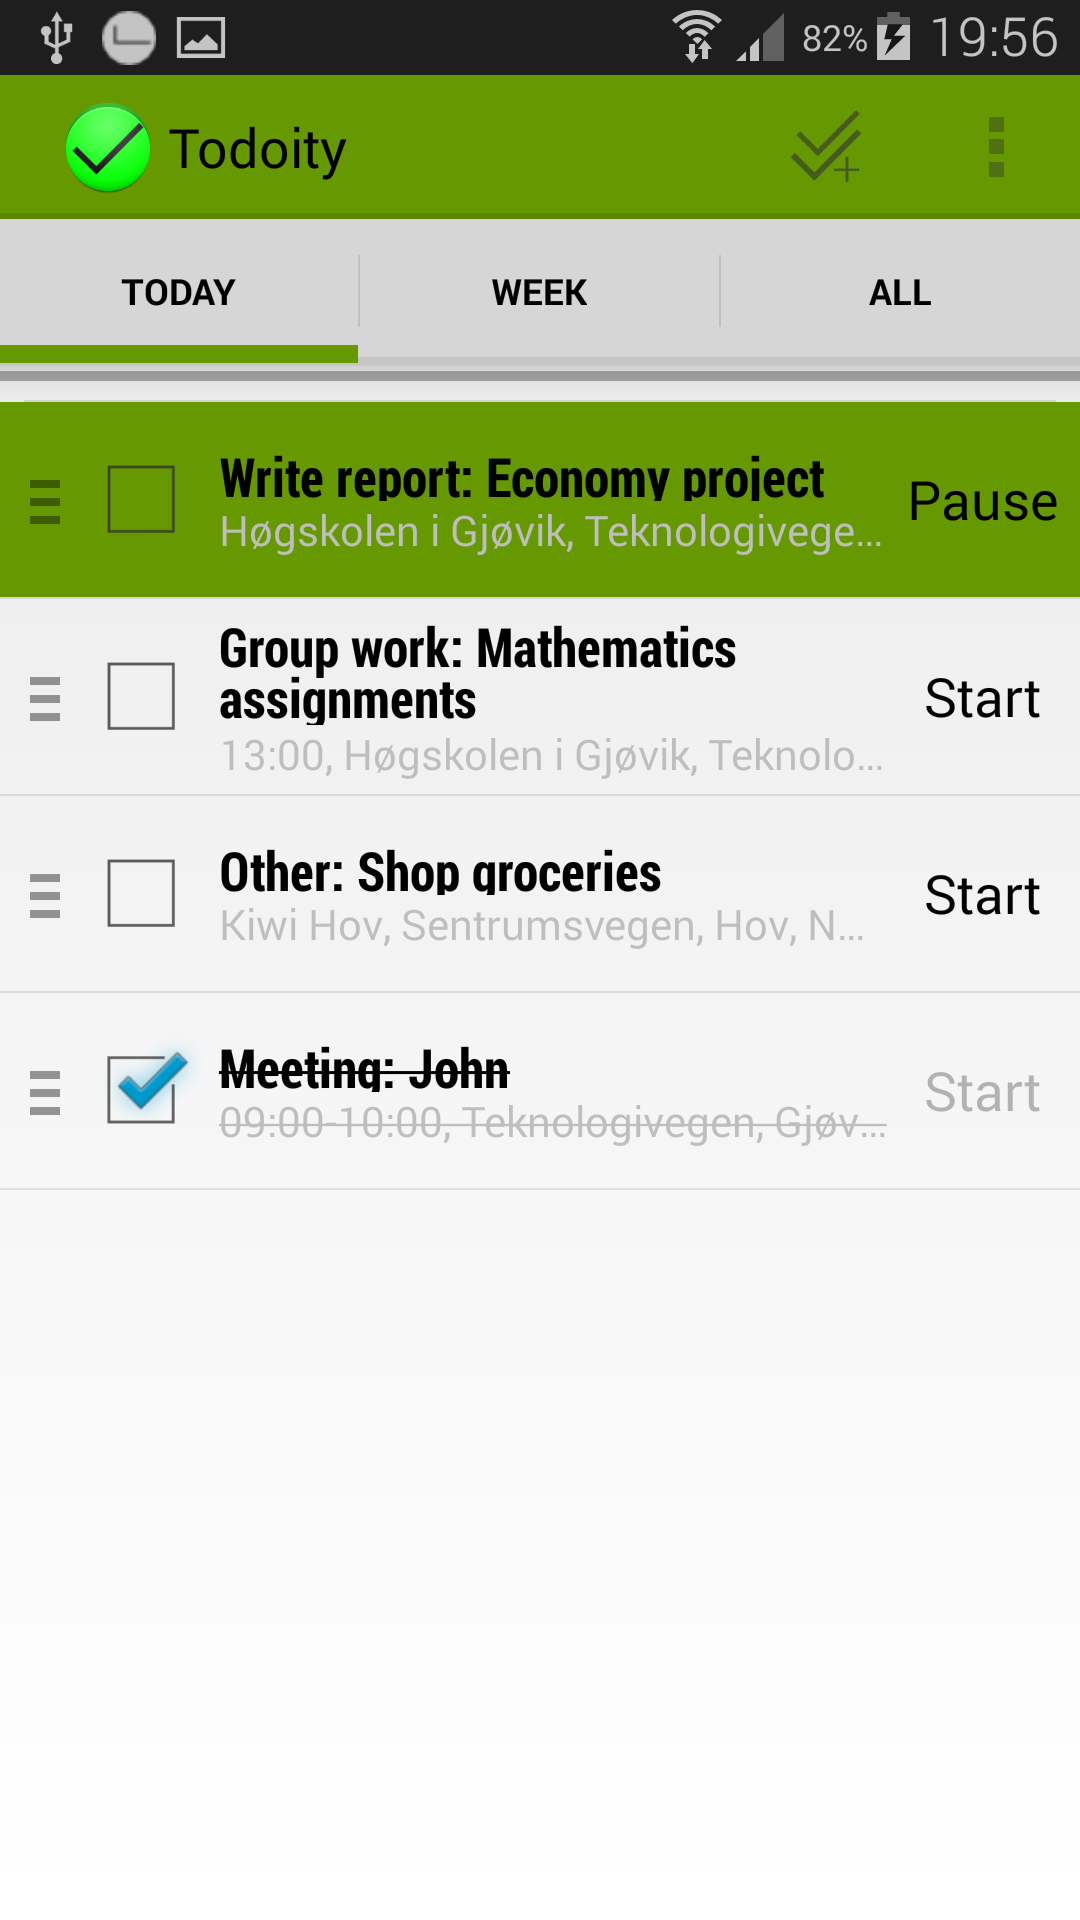
\includegraphics[width=0.5\textwidth]{figures/MainScreenStarted.png}
  \caption[Main application screen]{The main screen of the application, showing a few tasks where one is ongoing and one is finished.}
  \label{fig:designmainscreen}
\end{figure}


\subsection{Context acquisition}
By storing contextual information about how tasks are performed, the recommender will be able to not only provide recommendations based on current and planned contexts, but also take into account in what contexts tasks have been done previously. A certain task may work well in one context and poorly in another. However, before designing the overall schema of context representation, decisions on what contexts to actually use and collect needs to be made. In a mobile device there are typically many types of contexts that can be  collected via the system and its sensors. Some of these are:
\begin{itemize}
	\item Location
	\item Movement
	\item Time
	\item Activity
	\item Air pressure
	\item Ambient sound
	\item Humidity
	\item Orientation of device
\end{itemize}

Although all of these contexts, and more, could be collected by a mobile device, not all of them would be equally relevant to use in a to-do list application. While each of the contexts could be used to some degree, there are situations were some contexts would be redundant. Humidity, for example, could be a somewhat useful context for someone working on very specific tasks in very specific environments, say an environmentalist taking water samples near lakes and rivers. However, for students in an educational environment, such contexts are less relevant.

The actual contexts that was decided to be collected in the app were:
\begin{itemize}
	\item \emph{Location:} Both the planned location of the task as well as the actual location of where the task is performed is stored.
	\item \emph{Activity:} The movement of the device while contexts are collected.
	\item \emph{Time:} Each task is given timestamps both when they are started and ended. By doing this it is possible for the recommender to separate tasks that are done at specific times of the day, week or even month. Time spent doing a task is also tracked, as this may differ from the difference between the start and end times (users may pause doing a task).
\end{itemize}

The actual logic behind the tracking of tasks and their contexts is a separate problem. It was decided that the tracking if tasks would have to be manually started and stopped by the users. This was done by providing a start button for each task, as shown in Figure~\ref{fig:taskrepresentation}.
\begin{figure}[tbp]
  \centering
  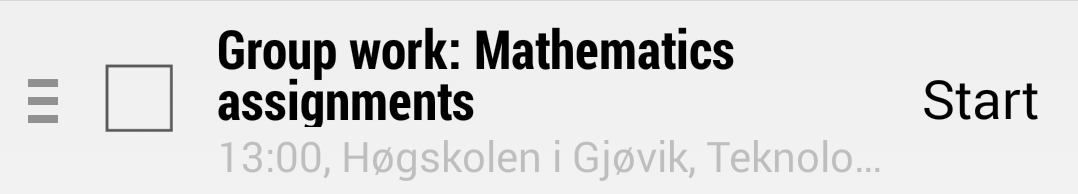
\includegraphics[width=0.5\textwidth]{figures/TaskRepresentation.png}
  \caption[In-app representation of task]{The in-app representation of a planned task.}
  \label{fig:taskrepresentation}
\end{figure} 

\subsection{Context storage}
A database was needed to store both the collected contexts and the tasks. Both an internal and external database was chosen to hold the data. An internal database was chosen because it is easy to implement as well as it allows for the application to be used while being offline. However, in order to easily retrieve and analyze the collected tasks and contexts for the thesis results, an external database was chosen. While the internal database only holds information regarding the specific installation, the external database holds all the information about all installations.

While many studies have looking into context modeling and representation (reference here), we decided to go with a normalized database approach. Context modeling and representation studies is often about providing proper abstraction from the raw context data. However, by using the integrated features for collecting contexts in Android, such abstractions are already built into the framework. The representation of the data is shown in Figure~\ref{fig:databasemodel} and Figure~\ref{fig:databasemodelexternal}

\begin{figure}[tbp]
  \centering
  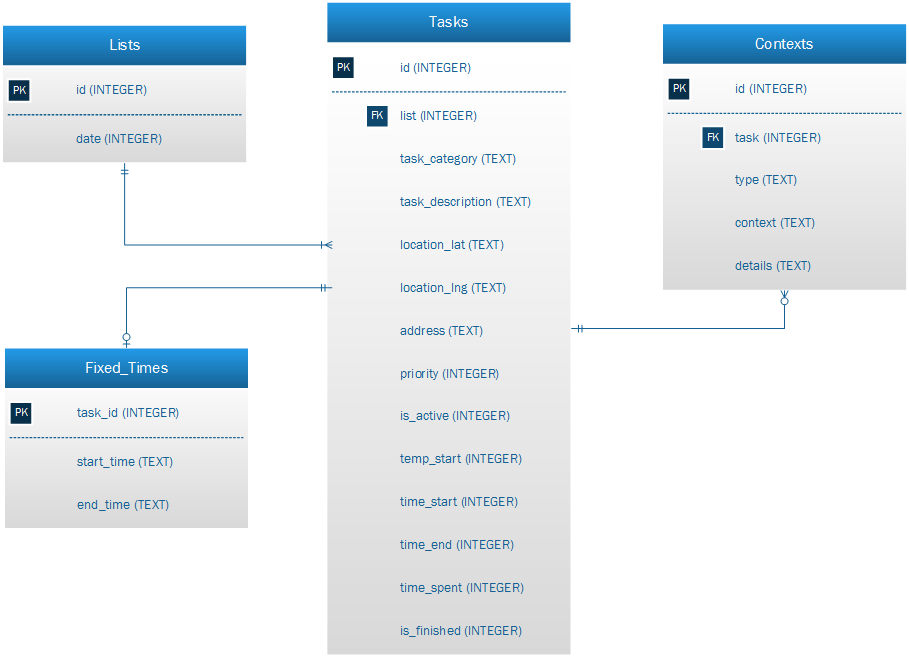
\includegraphics[width=\textwidth]{figures/DatabaseModel.png}
  \caption[Database model]{SQLite representation of the individual installations application data.}
  \label{fig:databasemodel}
\end{figure}

\begin{figure}[tbp]
  \centering
  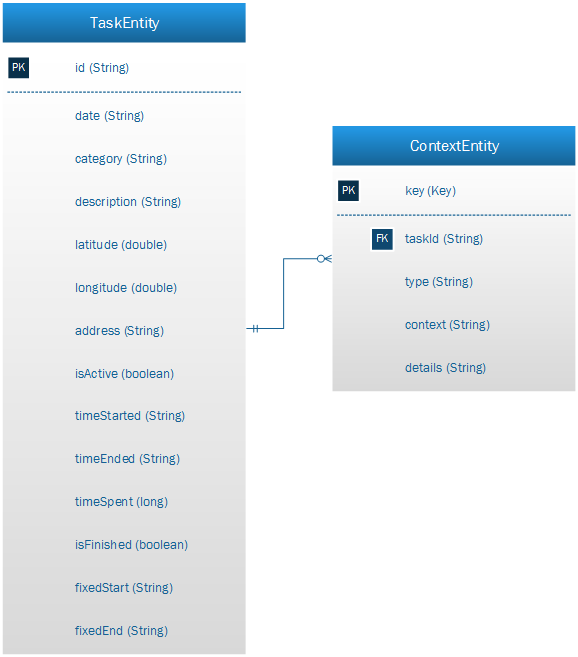
\includegraphics[width=0.5\textwidth]{figures/DatabaseModel_external.png}
  \caption[External database model]{The Google AppEngine datastore representation for all installations application data.}
  \label{fig:databasemodelexternal}
\end{figure}




\section{Recommender}
\label{sec:recommender}

When creating the recommender-part of the application, several decisions needed to be made. First of all, we needed to decide what kind of recommendations to make. There where many possible ways to do this:
\begin{itemize}
	\item Location proximity recommendations.
  \item Recommendations based on time of day.
  \item Recommendations based on time spent on previous tasks.
  \item Recommend tasks with fixed starting times.
  \item Recommend tasks based on the shortest traveling distance between tasks.
  \item Recommendations based on regularity of task occurrences.
  \item Combinations of the above.
\end{itemize}

After deciding what to recommend, the underlying logic also needs to be decided. A recommender will need some form of logic for comparison, so that it can know that it should recommend one task over another. Such logic already exist in some systems. We have seen Netflix\cite{netflix} recommending movies and Amazon\cite{amazon} recommending books and other wares. It is necessary to analyze these systems for potentially reusable recommendation algorithms:

\subsubsection{Neural networks}
Neural networks describes the process in which the computer\ldots
(half a page with a couple of references\ldots)

\subsubsection{Probability calculations}
The second approach is to use probability calculations to perform the recommendations. This is the approach that was decided to be used in this project. (some general information + a couple of references\ldots)

Unfinished \ldots

\subsection{Chosen recommendation algorithm}

As mentioned earlier, the input for the recommender consist of the users planned task, the current context, and the entire task history with related contexts. The recommender starts by looking at the categories of the user's planned tasks and tries to calculate a probability for each of them, representing how likely the task is going to be chosen next by the user. This calculation is done based on the tasks that the user has previously done and in what contexts. Probability calculations are made individually for each of the different contexts, but also for combinations of them. For example, the recommender will consider the current time of day and then find other tasks that have been done during the same time of day previously. The probability for a specific task is then calculated by dividing the number of occurrences of that particular task by the total number of tasks performed at that time of day. This is done for each of the tasks that the user has planned and the result is put into a hashmap, as shown in Table~\ref{tab:probabilitymaptimeofday}.
\begin{table}[tbp]
  \centering
  \begin{tabular}{|l|r|}
	\hline
	\textbf{Task category} & \textbf{Probability} \\
	\hline
	Attend lecture & 0.11 \\
  \hline
	Other & 0.24 \\
	\hline
	Practical work & 0.46 \\
	\hline
	Read & 0.14 \\
	\hline
	Write report & 0.05 \\
	\hline
  \end{tabular}
  \caption{Example recommendation probability hashmap}
  \label{tab:probabilitymaptimeofday}
\end{table}

The same process is executed for other contexts as well. For example, based on the current location of the user, the recommender finds all tasks that have been performed in that particular location. Probabilities are then calculated the same way as for the time of day. The task probability hashmap based on location may look like Table~\ref{probabilitymaplocation}.
\begin{table}[tbp]
  \centering
  \begin{tabular}{|l|r|}
	\hline
	\textbf{Task category} & \textbf{Probability} \\
	\hline
	Attend lecture & 0.41 \\
	\hline
	Other & 0.13 \\
	\hline
	Practical work & 0.25 \\
	\hline
	Read & 0.16 \\
	\hline
	Write report & 0.05 \\
	\hline
  \end{tabular}
  \caption{Location recommendation probability hashmap}
  \label{tab:probabilitymaplocation}
\end{table}

Similar hashmaps are calculated for each context and all combinations of them. This means:
\begin{itemize}
	\item Time of day
	\item Day of week
	\item Location
	\item Time of day \emph{and} location
	\item Time of day \emph{and} day of week
	\item Day of week \emph{and} location
	\item Time of day \emph{and} day of week \emph{and} location
\end{itemize}
The highest probability from each of these individual probability hashmaps are then put into a resulting hashmap, where the highest probability in will be the actual task recommendation med by the recommender. Looking at Table~\ref{tab:probabilitymaptimeofday} and Table~\ref{tab:probabilitymaplocation}, the resulting hashmap will look like Table~\ref{tab:probabilitymapresult}.
\begin{table}[tbp]
  \centering
  \begin{tabular}{|l|r|}
	\hline
	\textbf{Task category} & \textbf{Probability} \\
	\hline
	Attend lecture & 0.41 \\
	\hline
	Practical work & 0.46 \\
	\hline
  \end{tabular}
  \caption{Resulting probability hashmap upon which the actual recommendation is made}
  \label{tab:probabilitymapresult}
\end{table}
The actual recommendation made by the recommender in this example would be the task with the category ``practical work''.
